\documentclass[12pt,a4paper]{article}

% ─── Packages ────────────────────────────────────────────────────────────────
\usepackage[utf8]{inputenc}
\usepackage[T5]{fontenc}
\usepackage[vietnamese,english]{babel}
\usepackage{amsmath, amssymb, mathtools}
\usepackage{graphicx}
\usepackage{float}
\usepackage{booktabs}
\usepackage{array}
\usepackage{xcolor}
\usepackage{listings}
\usepackage{hyperref}
\usepackage{geometry}
\usepackage{caption}
\usepackage{subcaption}
\usepackage{enumitem}
\usepackage{titlesec}
\usepackage{fancyhdr}
\usepackage{parskip}

\geometry{margin=2.5cm}

% ─── Code style ──────────────────────────────────────────────────────────────
\lstdefinestyle{python}{
  language=Python,
  basicstyle=\ttfamily\small,
  keywordstyle=\color{blue!70!black}\bfseries,
  commentstyle=\color{green!50!black}\itshape,
  stringstyle=\color{red!60!black},
  numberstyle=\tiny\color{gray},
  numbers=left,
  stepnumber=1,
  frame=single,
  breaklines=true,
  tabsize=4,
  showstringspaces=false,
  backgroundcolor=\color{gray!8},
}
\lstset{style=python}

% ─── Header / Footer ─────────────────────────────────────────────────────────
\pagestyle{fancy}
\fancyhf{}
\rhead{MAT3562E -- Computer Vision Lab 03}
\lhead{Bui Quang Chien -- 23001837}
\cfoot{\thepage}

% ─── Hyperref ────────────────────────────────────────────────────────────────
\hypersetup{
  colorlinks=true,
  linkcolor=blue!60!black,
  urlcolor=blue,
}

% ─── Title ───────────────────────────────────────────────────────────────────
\title{%
  \textbf{LAB 03 REPORT}\\[0.4em]
  \large Spatial \& Frequency Domain Processing:\\
  Mini-Project --- Image Enhancement Pipeline \\[0.8em]
  \normalsize MAT3562E -- Computer Vision\\
  Academic Year 2025--2026
}
\author{
  Bui Quang Chien\\
  MSSV: 23001837
}
\date{March 2026}

% ─────────────────────────────────────────────────────────────────────────────
\begin{document}
\maketitle
\tableofcontents
\newpage

% =============================================================================
\section{Overview and Learning Objectives}
% =============================================================================

This lab covers the following topics across nine modules:

\begin{itemize}[leftmargin=*]
  \item \textbf{Module 1--2:} Frequency domain fundamentals --- DFT/FFT, magnitude spectrum analysis, and ideal low-pass / high-pass frequency filters.
  \item \textbf{Module 3:} Discrete convolution --- custom 2D convolution vs.\ OpenCV \texttt{filter2D}, padding effects.
  \item \textbf{Module 4:} Smoothing filters --- mean filter, Gaussian filter, effect of kernel size and $\sigma$.
  \item \textbf{Module 5:} Denoising pipeline --- comparing mean, Gaussian, and median filters on Gaussian noise and salt-\&-pepper noise.
  \item \textbf{Module 6:} Sharpening --- Laplacian sharpening and unsharp masking.
  \item \textbf{Module 7:} Edge detection --- Sobel gradient operator and thresholding.
  \item \textbf{Module 8:} Canny edge detection --- full 5-step pipeline (Gaussian smoothing, Sobel gradient, NMS, double threshold, hysteresis).
  \item \textbf{Module 9:} Spatial vs.\ frequency domain filtering comparison (convolution theorem).
  \item \textbf{Mini-Project:} Build an end-to-end image enhancement pipeline integrating all learned modules.
\end{itemize}

The \textbf{Mini-Project} (Module~13) is the main deliverable of this report. It integrates noise injection, denoising, sharpening, and edge detection into a single configurable pipeline.

% =============================================================================
\section{Environment and Common Utilities}
% =============================================================================

All code runs in Python~3.12 with the following packages:
\texttt{numpy 2.4}, \texttt{opencv-python 4.13}, \texttt{matplotlib 3.10}.

\begin{lstlisting}
import numpy as np
import cv2
import matplotlib.pyplot as plt
\end{lstlisting}

The following helper functions were defined earlier in the lab and are reused by the mini-project:

\begin{lstlisting}
def show_gray(title, img):
    plt.figure(figsize=(5,4))
    plt.imshow(img, cmap='gray')
    plt.title(title); plt.axis('off'); plt.show()

def conv2d_same(image, kernel):
    """2D convolution with zero-padding (same size output)."""
    image = image.astype(np.float64)
    kernel = kernel.astype(np.float64)
    kh, kw = kernel.shape
    pad_h, pad_w = kh//2, kw//2
    padded = np.pad(image, ((pad_h,pad_h),(pad_w,pad_w)),
                    mode='constant')
    H, W = image.shape
    out = np.zeros((H, W), dtype=np.float64)
    for i in range(H):
        for j in range(W):
            out[i, j] = np.sum(padded[i:i+kh, j:j+kw] * kernel)
    return out
\end{lstlisting}

% =============================================================================
\section{Mini-Project: Image Enhancement Pipeline}
% =============================================================================

\subsection{Objective}

Build a simple yet complete image enhancement pipeline that demonstrates mastery of the learned modules. The pipeline takes a clean grayscale image and processes it through four stages:

\begin{enumerate}
  \item \textbf{Noise injection} --- add synthetic noise (Gaussian or salt-\&-pepper).
  \item \textbf{Denoising} --- remove the injected noise using an appropriate filter.
  \item \textbf{Sharpening} --- enhance edges using unsharp masking.
  \item \textbf{Edge detection} --- extract edge maps using Canny.
\end{enumerate}

\subsection{Pipeline Design}

Two parallel pipelines are evaluated, one for each noise type:

\begin{table}[H]
  \centering
  \begin{tabular}{@{}llll@{}}
    \toprule
    \textbf{Stage} & \textbf{Gaussian Pipeline} & \textbf{Salt-\&-Pepper Pipeline} \\
    \midrule
    1. Noise & Gaussian ($\sigma=25$) & Salt-\&-pepper ($p=0.03$) \\
    2. Denoise & GaussianBlur $(5\times5,\;\sigma=1.0)$ & MedianBlur $(5\times5)$ \\
    3. Sharpen & Unsharp masking ($k=1.0$) & Unsharp masking ($k=1.0$) \\
    4. Edge & Canny ($T_\text{low}=30,\;T_\text{high}=80$) & Canny ($T_\text{low}=30,\;T_\text{high}=80$) \\
    \bottomrule
  \end{tabular}
  \caption{Pipeline configurations for each noise type.}
  \label{tab:pipeline}
\end{table}

\subsection{Implementation}

\subsubsection*{Step 1: Noise Injection}

\begin{lstlisting}
def add_gaussian_noise(image, sigma=20):
    noise = np.random.normal(0, sigma, image.shape)
    noisy = image.astype(np.float64) + noise
    return np.clip(noisy, 0, 255).astype(np.uint8)

def add_salt_pepper(image, prob=0.02):
    out = image.copy()
    rnd = np.random.rand(*image.shape)
    out[rnd < prob/2] = 0          # salt
    out[rnd > 1 - prob/2] = 255    # pepper
    return out
\end{lstlisting}

\textbf{Gaussian noise} adds i.i.d.\ samples from $\mathcal{N}(0, \sigma^2)$ to each pixel. \textbf{Salt-\&-pepper noise} randomly replaces a fraction $p$ of pixels with extreme values (0~or~255).

\subsubsection*{Step 2: Denoising}

\begin{lstlisting}
# Gaussian pipeline
denoised_gauss = cv2.GaussianBlur(noisy_gauss, (5,5), 1.0)
# Salt-&-pepper pipeline
denoised_sp = cv2.medianBlur(noisy_sp, 5)
\end{lstlisting}

\subsubsection*{Step 3: Sharpening (Unsharp Masking)}

Unsharp masking computes a high-frequency mask by subtracting a blurred version from the denoised image, then adds it back with strength $k$:

\begin{equation}
  g_\text{sharp}(x,y) = f(x,y) + k \cdot \bigl[ f(x,y) - f_\text{blur}(x,y) \bigr]
  \label{eq:unsharp}
\end{equation}

\begin{lstlisting}
blur_tmp = cv2.GaussianBlur(denoised, (5,5), 1.0)
hf_mask = denoised.astype(np.float64) - blur_tmp.astype(np.float64)
sharp = np.clip(denoised.astype(np.float64) + k * hf_mask,
                0, 255).astype(np.uint8)
\end{lstlisting}

\subsubsection*{Step 4: Edge Detection (Canny)}

\begin{lstlisting}
edges = cv2.Canny(sharp, 30, 80)
\end{lstlisting}

OpenCV's Canny implementation performs: Gaussian smoothing $\to$ Sobel gradient $\to$ non-maximum suppression $\to$ double threshold $\to$ hysteresis tracking.

\subsubsection*{Full Pipeline Code}

\begin{lstlisting}
img_clean = img_edge.copy()   # lena.png grayscale

# --- Gaussian noise pipeline ---
noisy_gauss = add_gaussian_noise(img_clean, sigma=25)
denoised_gauss = cv2.GaussianBlur(noisy_gauss, (5,5), 1.0)
blur_tmp = cv2.GaussianBlur(denoised_gauss, (5,5), 1.0)
hf_mask = denoised_gauss.astype(np.float64) \
        - blur_tmp.astype(np.float64)
sharp_gauss = np.clip(
    denoised_gauss.astype(np.float64) + 1.0 * hf_mask,
    0, 255).astype(np.uint8)
edges_gauss = cv2.Canny(sharp_gauss, 30, 80)

# --- Salt-&-pepper pipeline ---
noisy_sp = add_salt_pepper(img_clean, prob=0.03)
denoised_sp = cv2.medianBlur(noisy_sp, 5)
blur_tmp2 = cv2.GaussianBlur(denoised_sp, (5,5), 1.0)
hf_mask2 = denoised_sp.astype(np.float64) \
         - blur_tmp2.astype(np.float64)
sharp_sp = np.clip(
    denoised_sp.astype(np.float64) + 1.0 * hf_mask2,
    0, 255).astype(np.uint8)
edges_sp = cv2.Canny(sharp_sp, 30, 80)
\end{lstlisting}

% ─────────────────────────────────────────────────────────────────────────────
\subsection{Results}
% ─────────────────────────────────────────────────────────────────────────────

Figure~\ref{fig:pipeline} shows the complete visual grid for both pipelines.

\begin{figure}[H]
  \centering
  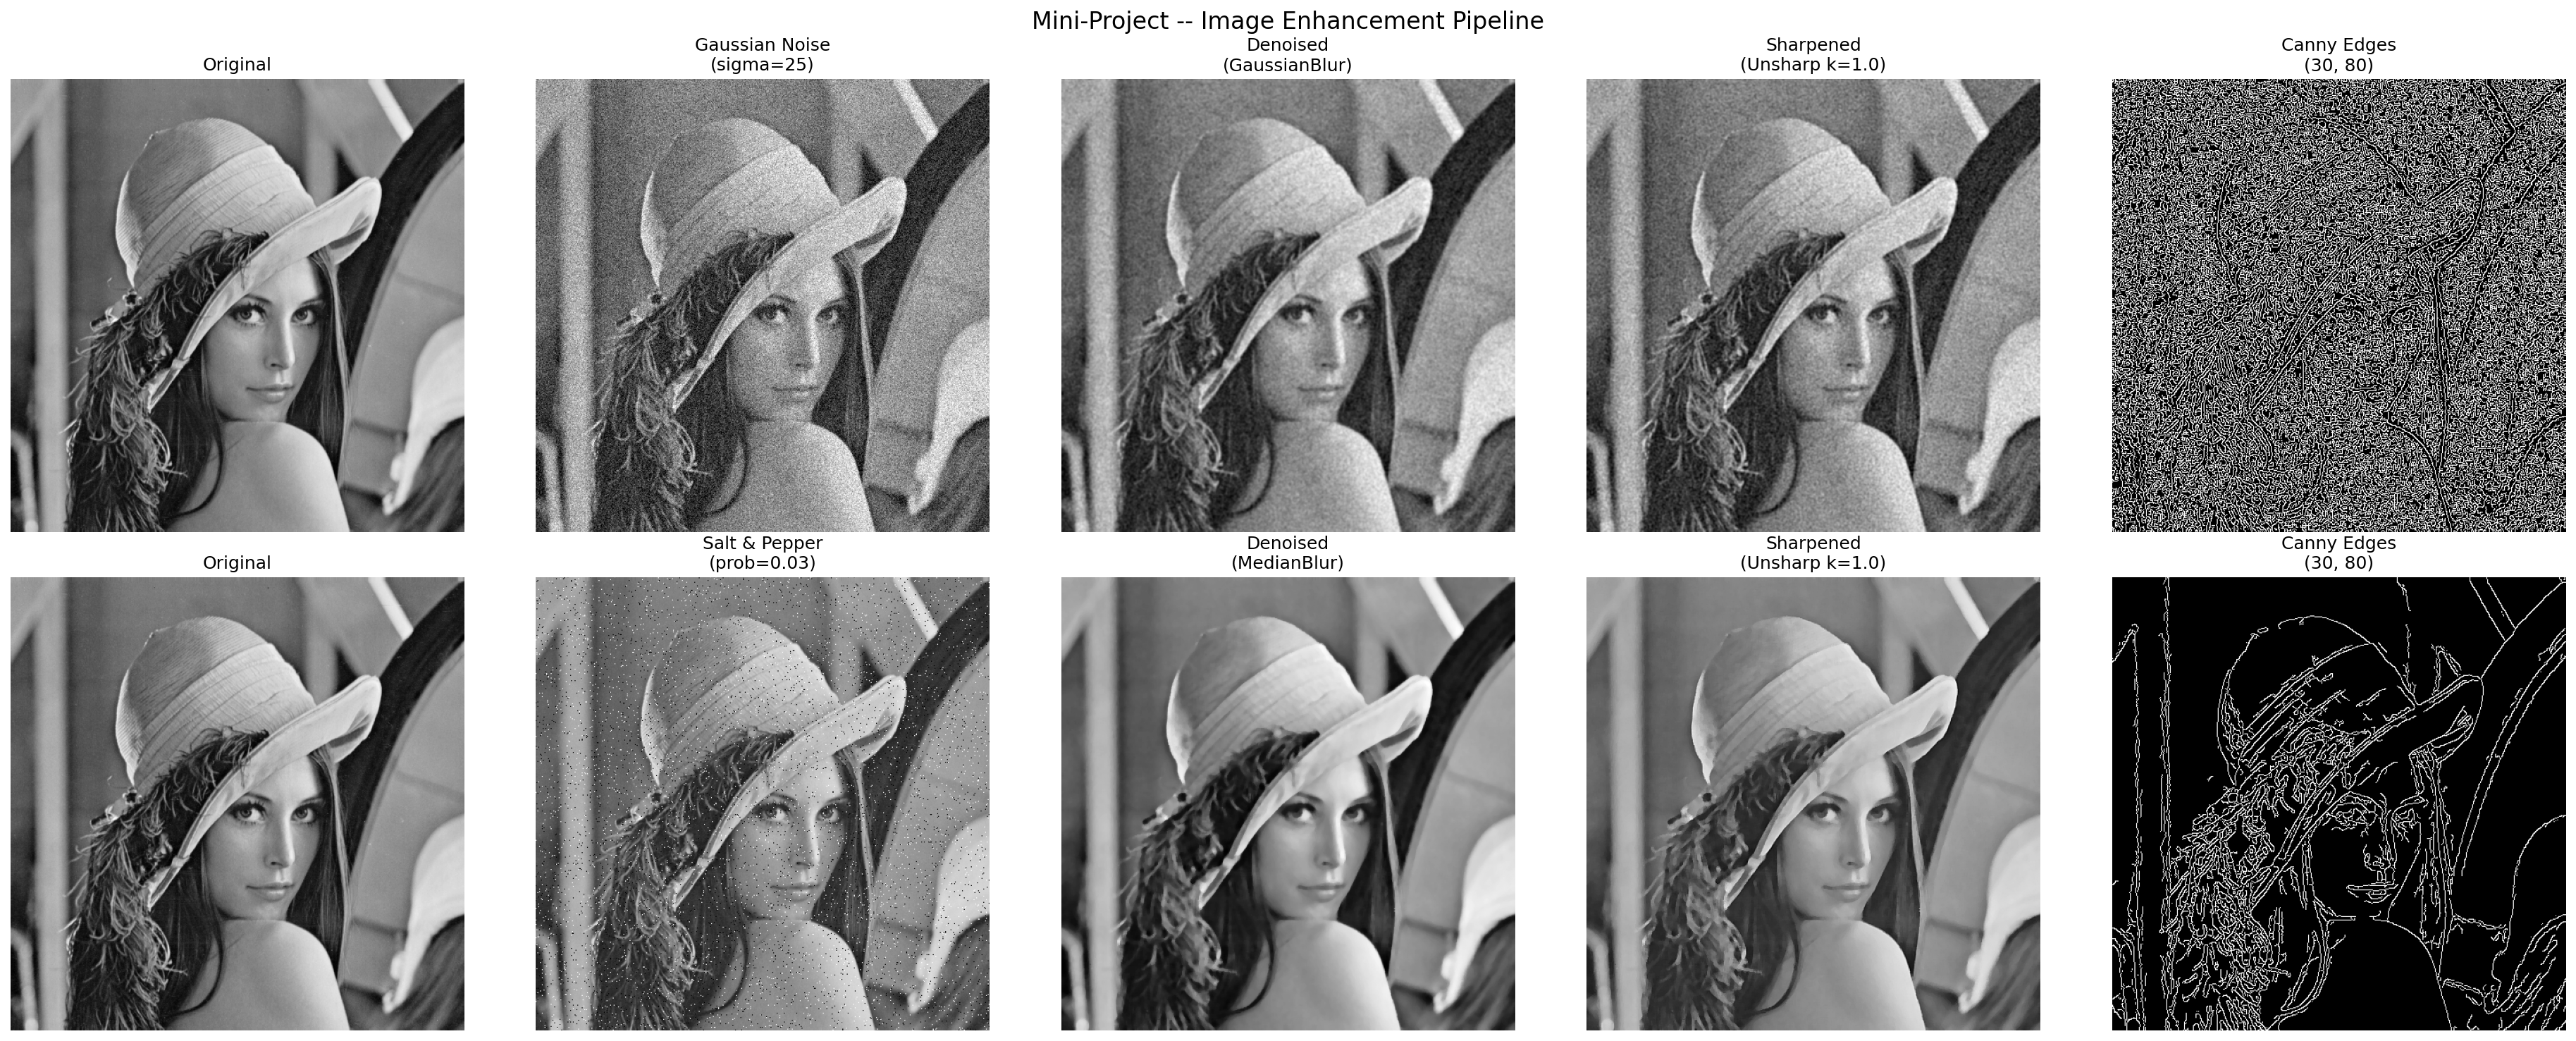
\includegraphics[width=\textwidth]{data/report_figs/mini_project_pipeline.png}
  \caption{Mini-Project --- Image Enhancement Pipeline. \textbf{Top row:} Gaussian noise ($\sigma=25$) pipeline. \textbf{Bottom row:} Salt-\&-pepper noise ($p=0.03$) pipeline. Columns from left to right: original, noisy, denoised, sharpened, Canny edge map.}
  \label{fig:pipeline}
\end{figure}

\textbf{Key observations from the visual grid:}

\begin{itemize}[leftmargin=*]
  \item The Gaussian pipeline (top row) shows that GaussianBlur effectively reduces the noise spread, but residual noise is still visible after sharpening. The Canny edge map captures many false edges from amplified noise.
  \item The salt-\&-pepper pipeline (bottom row) shows that MedianBlur cleanly removes the impulse noise. The resulting edge map is much cleaner, with continuous contours.
\end{itemize}

% ─────────────────────────────────────────────────────────────────────────────
\subsection{Analysis}
% ─────────────────────────────────────────────────────────────────────────────

\subsubsection{Q1: Which denoising filter is most suitable for each noise type? Why?}

\begin{itemize}[leftmargin=*]
  \item \textbf{Gaussian noise $\to$ Gaussian filter:} Gaussian noise is \emph{additive} and \emph{normally distributed} across all pixels. A Gaussian low-pass filter averages out the noise while preserving edge structure better than a mean filter (thanks to the weighted kernel). The matched distribution between the noise model and the filter's frequency response makes this pairing optimal.

  \item \textbf{Salt-\&-pepper noise $\to$ Median filter:} Salt-\&-pepper is \emph{impulse} noise --- a small fraction of pixels are replaced by extreme values (0 or 255). Linear filters (mean, Gaussian) spread these outliers into neighbouring pixels, creating grey ``halos''. The median filter replaces each pixel with the \emph{median} of its neighbourhood, which is inherently robust to outliers: the extreme 0/255 values are discarded because they always fall at the ends of the sorted window.
\end{itemize}

\subsubsection{Q2: Which sharpening method produces fewer artefacts? Why?}

\textbf{Unsharp masking} produces fewer artefacts than Laplacian sharpening at comparable enhancement levels, for two reasons:

\begin{enumerate}
  \item The Gaussian blur step in unsharp masking acts as a \emph{built-in noise suppressor}. The high-frequency mask $\text{HF} = f - f_\text{blur}$ captures edge information \emph{after} the noise has been partially smoothed, so less noise is amplified.

  \item The Laplacian operator is a second-order derivative --- it is extremely sensitive to rapid intensity changes, amplifying noise and fine texture indiscriminately. Even at moderate $\lambda$ values ($\geq 1.0$), ``halo'' artefacts and noise grains become visible.
\end{enumerate}

In the pipeline, unsharp masking with $k = 1.0$ enhances edges effectively while keeping artefacts minimal.

\subsubsection{Q3: How do parameter changes affect the edge map?}

The final Canny edge map is the cumulative result of all upstream parameters. The interactions can be summarised as:

\begin{table}[H]
  \centering
  \small
  \begin{tabular}{@{}p{3.8cm}p{5cm}p{5cm}@{}}
    \toprule
    \textbf{Parameter change} & \textbf{Effect on image} & \textbf{Effect on edge map} \\
    \midrule
    Increase denoise strength (larger kernel / $\sigma$) &
      Smoother image, fine details lost &
      Fewer false edges, but weak true edges may disappear \\
    \addlinespace
    Increase sharpening strength ($k$ or $\lambda$) &
      Sharper edges, but noise amplified &
      More edges detected (both true and false) \\
    \addlinespace
    Increase Canny thresholds ($T_\text{low}$, $T_\text{high}$) &
      --- &
      Only strong edges retained; cleaner but incomplete contours \\
    \addlinespace
    Decrease Canny thresholds &
      --- &
      More edges including weak/noisy ones; better connectivity but noisier \\
    \bottomrule
  \end{tabular}
  \caption{Impact of parameter changes on the final edge map.}
  \label{tab:param}
\end{table}

\textbf{Key insight:} There is a three-way trade-off between denoising strength, sharpening strength, and Canny thresholds. Optimal results require balancing all three: denoise just enough to suppress noise without destroying edges, sharpen moderately to restore edge contrast, and tune Canny thresholds to match the resulting gradient distribution.

% =============================================================================
\section{Conclusion}
% =============================================================================

This lab provided a comprehensive journey through spatial and frequency domain image processing:

\begin{itemize}[leftmargin=*]
  \item The \textbf{frequency domain} perspective (DFT/FFT, ideal LPF/HPF) reveals that low-frequency components control smooth intensity variation while high-frequency components encode edges and texture.
  \item \textbf{Convolution} in the spatial domain is equivalent to multiplication in the frequency domain (convolution theorem).
  \item \textbf{Denoising} must be matched to the noise model: Gaussian filter for Gaussian noise, median filter for impulse noise.
  \item \textbf{Sharpening} via unsharp masking is more controllable and less artefact-prone than direct Laplacian enhancement.
  \item \textbf{Edge detection} with Canny provides robust, thin edge maps when parameters are tuned to the image's noise level and edge strength.
  \item The \textbf{mini-project} demonstrated that building an effective image enhancement pipeline requires careful parameter tuning at each stage --- no single ``best'' configuration exists; the optimal settings depend on the specific noise characteristics and the downstream task.
\end{itemize}

\end{document}
